\documentclass[a4paper, 12pt]{report}
\usepackage[utf8]{inputenc}
\usepackage{tikz}
\usepackage{graphicx}
\usepackage{geometry}
\usetikzlibrary{calc,patterns,angles,quotes}
\geometry{margin=1in,left=0.6in,right=0.6in,bottom=0.5in}
\usepackage{fancyhdr}
\usepackage{hyperref}
\usepackage{chemfig}
\usetikzlibrary{calc}
\usepackage{enumitem}
\usepackage{placeins}
\usepackage{caption}
\usepackage{array}
\usepackage{float}
\usepackage{amsmath, amssymb, amscd, MnSymbol,mathrsfs}
\usepackage{tcolorbox}
\usepackage{bibref}
\usepackage{bm}
\newcommand{\vect}[1]{\boldsymbol{\mathbf{#1}}}
\usepackage{pdfpages}

\usepackage{empheq}
\usepackage{pgfplots}
\pgfplotsset{compat=1.18}
\usetikzlibrary{calc, angles, quotes}
\usepackage[oldvoltagedirection]{circuitikz}
\usepackage{booktabs}
\usepackage{array}
\usepackage{arydshln}
\usepackage{tcolorbox}

\usepackage{hyperref}
\usepackage{cancel}
\usepackage{changepage}
\usepackage{placeins}
\usepackage{enumitem}
\usepackage{pgf}
\usetikzlibrary{decorations.markings}
\usetikzlibrary{decorations.pathmorphing}
\usepackage{tikz-3dplot}

\renewcommand{\thechapter}{\Alph{chapter}} % Use letters for parts
\renewcommand{\chaptername}{Part} % Change "Chapter" to "Part"
\renewcommand{\thesection}{\Alph{chapter}.\arabic{section}} % Use letters for sections

\usepackage{listings}
\usepackage{bm}
\usepackage{minted}

\usepackage{courier}
\usepackage{xcolor}
\usepackage{color}
\def\ni{green!60!black!40!white}

\lstdefinestyle{mypythonstyle}{
    language=Python,
    basicstyle=\footnotesize\ttfamily,
    numbers=left,
    numberstyle=\tiny,
    numbersep=9pt,
    showstringspaces=false,
    frame=single,
    breaklines=true,
    keywordstyle=\color{blue!80!black}\bfseries,  % Darker blue and bold for keywords
    commentstyle=\color{green!60!black},  % Softer gray for comments
    stringstyle=\color{orange},  % Different color for strings
    backgroundcolor=\color{gray!5},  % Light gray for background
    tabsize=4,
    belowcaptionskip=10pt, % Adjust space below caption
    morecomment=[l]{//},  % For inline comments
    literate={~} {$\sim$}{1},  % Converts tilde to a symbol
}

\usepackage{xcolor}
\definecolor{light-gray}{gray}{0.9}
\newcommand{\code}[1]{\colorbox{light-gray}{\texttt{#1}}}

\lstdefinestyle{matlab}{
    language=MATLAB,
    basicstyle=\ttfamily\footnotesize,
    breaklines=true,
    commentstyle=\color{green!60!black},
    keywordstyle=\color{blue!80!black}\bfseries,
    stringstyle=\color{red!70!black},
    numberstyle=\tiny\color{gray},
    frame=single,
    framesep=5pt,
    rulecolor=\color{black!30},
    backgroundcolor=\color{white!94!gray},
    emphstyle=\color{purple}\bfseries,
    emph={[2]\%},
    emphstyle={[2]\color{green!60!black}},
    showstringspaces=false,
    tabsize=4,
    belowcaptionskip=10pt, % Adjust space below caption
    morekeywords={import,classdef,properties,methods,end,
        function,return,if,else,elseif,switch,case,otherwise,
        for,while,break,continue,try,catch,global,persistent},
    morecomment=[l][\color{magenta!70!black}]{\%\%},
    morestring=[b]',
    literate=
    *{0}{{{\color{cyan!70!black}0}}}1
    {1}{{{\color{cyan!70!black}1}}}1
    {2}{{{\color{cyan!70!black}2}}}1
    {3}{{{\color{cyan!70!black}3}}}1
    {4}{{{\color{cyan!70!black}4}}}1
    {5}{{{\color{cyan!70!black}5}}}1
    {6}{{{\color{cyan!70!black}6}}}1
    {7}{{{\color{cyan!70!black}7}}}1
    {8}{{{\color{cyan!70!black}8}}}1
    {9}{{{\color{cyan!70!black}9}}}1
}

\def\link{blue!50!black}
\makeatletter
\renewcommand*\env@matrix[1][\arraystretch]{%
    \edef\arraystretch{#1}%
    \hskip -\arraycolsep
    \let\@ifnextchar\new@ifnextchar
    \array{*{\c@MaxMatrixCols}c}
}
\makeatother
\usepackage{tabularray}

\pagestyle{fancy}
\fancyhf{}
\fancyhead[L]{Module: EG4017 - Engineering Mathematics}
\fancyhead[R]{Page \thepage}
\usepackage{datetime}


\title{\vspace{3em} \Huge \textbf{Engineering\\ Mathematics and Computing}\\ \vspace{1em} \Large Task 2: Coursework Assessment}
\author{Student Name: Sakariye Abiikar\\ KID: 2371673}
\date{Last Updated: \today,\
     \currenttime\\ Submission Deadline: Thursday \(9^{\text{th}}\) January, 2025, 5pm \\[1em] Git Repo : \color{blue}\url{https://github.com/sakx7/mathcompuni2}}

\newtheorem{theorem}{Theorem}[section]
\newtheorem{lemma}[theorem]{Lemma}

\begin{document}
    
    \maketitle
    \thispagestyle{empty}
    
    \newpage
    \thispagestyle{empty}
    \newgeometry{margin=1in,left=0.6in,right=0.6in,bottom=0in}
    
    \chapter{Mathematics}
    
    \newpage\centering\restoregeometry
    
    \setcounter{page}{1}
    \fancyhead[L]{Part A: Mathematics}
    
    
    \begin{tcolorbox}[title={\color{black}\section{Q1}}, colback=white, colframe=\ni, boxrule=1mm, width=1\textwidth]
        1. Find \( \int \frac{1}{7x + 6} \, dx \)
    \end{tcolorbox}
    \[\int \frac{1}{7x + 6} \, dx\]
    Use substitution, Let 
    \[u = 7x + 6\]
    \[\frac{du}{dx} = 7 \quad \Rightarrow \quad dx = \frac{du}{7}\]
    Substituting into the integral, we get
    \[\int \frac{1}{7x + 6} \, dx = \frac{1}{7} \int \frac{1}{u} \, du\]
    This is a standard integral of the reciprocal
    \[\frac{1}{7} \int \frac{1}{u} \, du = \frac{1}{7} \ln |u| + C\]
    Finally, substituting \(u\) back in, we get
    \[\boxed{\int \frac{1}{7x + 6} \, dx = \frac{1}{7} \ln |7x + 6| + C}\]
    
    
    \newpage
    
    \begin{tcolorbox}[title={\color{black}\section{Q2}}, colback=white, colframe=\ni, boxrule=1mm, width=1\textwidth]
        2. Find \( \int \frac{x}{\sqrt{4 - x^2}} \, dx \)
    \end{tcolorbox}
    
    \[\int \frac{x}{\sqrt{4 - x^2}} \, dx\]
    Use substitution, Let\\[-1.5em] 
    \[u = 4 - x^2\]
    \[\frac{du}{dx} = -2x \quad \Rightarrow \quad dx = -\frac{du}{2x}\]
    Substituting into integral, we get
    \[\int \frac{x}{\sqrt{4 - x^2}} \, dx = \int \frac{x}{\sqrt{u}} \cdot \left(-\frac{du}{2x}\right) = -\frac{1}{2} \int \frac{1}{\sqrt{u}} \, du\]
    This is a standard integral of the power
    \[-\frac{1}{2} \int u^{-\frac{1}{2}} \, du = -\frac{1}{2} \cdot 2 \sqrt{u} + C = -\sqrt{u} + C\]
    Finally, substituting back \( u = 4 - x^2 \), we get
    \[\boxed{\int \frac{x}{\sqrt{4 - x^2}} \, dx = -\sqrt{4 - x^2} + C}\]
    
    
    
    \newpage
    
    \begin{tcolorbox}[title={\color{black}\section{Q3}}, colback=white, colframe=\ni, boxrule=1mm, width=1\textwidth]
        3. Obtain the general solution of the equation \( \frac{d^2 y}{dx^2} - 18 \frac{dy}{dx} + 81y = 0 \) 
    \end{tcolorbox}
    
    

    \[ \frac{d^2 y}{dx^2} - 18 \frac{dy}{dx} + 81y = 0 \]    
    We use the ansatz \( y = e^{rx} \), substituting it, along with its corresponding derivatives:
    \[r^2 e^{rx} - 18r e^{rx} + 81 e^{rx} = 0\]
    Dividing through by \( e^{rx} \) (which is never zero), we get the characteristic equation:
    \[ r^2 - 18r + 81 = 0 \]
    We can factorize the quadratic as:
    \[(r - 9)(r - 9) = 0 \]
    This gives us a repeated root:
    \[ r_1 = r_2 = 9 \]
    For a second-order linear homogeneous differential equation with constant coefficients and a repeated root \( r \), the general solution is:
    \[ y(x) = c_1 e^{rx} + c_2 x e^{rx} \]
    Substituting \( r = 9 \) into the general solution, we get:
    \[ y(x) = c_1 e^{9x} + c_2 x e^{9x} \]
    Factorising we get the final solution as:
    \[ \boxed{y(x) = e^{9x} (c_1 + c_2 x)} \]
    \textbf{Interval of validity}: Nothing really stands out, no singularities or undefined behaviours. Therefore, the interval of validity is:
    \[(-\infty, \infty) = \left\{x \in \mathbb{R} \;\; | -\infty < x < \infty\right\}\]
    This means the solution is valid for all real values of \(x\). The constant \(C\) does not effect the solutions validity regardless of its value.
       
    \newpage
    
    \begin{tcolorbox}[title={\color{black}\section{Q4}}, colback=white, colframe=\ni, boxrule=1mm, width=1\textwidth]
        4. Find the particular solution of the differential equation \( \frac{dy}{dx} + 3y x^3 = 0 \), given \( y(0) = 1 \)
    \end{tcolorbox}
    
    \[\frac{dy}{dx} + 3y x^3 = 0\]
    Separate the variables:
    \[\frac{1}{y} \, dy = -3x^3 \, dx\]
    Integrating both sides:
    \[\int \frac{1}{y} \, dy = \int -3x^3 \, dx\]
    \[\ln|y| = -\frac{3x^4}{4} + C\]
    Exponentiating both sides:
    \begin{align*}
        y=& \exp\left(-\frac{3x^4}{4} + C\right)\\
        y=& C \exp\left(-\frac{3x^4}{4}\right)
    \end{align*}
    Apply the initial condition \( y(0) = 1 \):
    \[1 = C \exp\left(-\frac{3(0)^4}{4}\right)\]
    \[C = 1\]
    Thus, the particular solution is:
    \[\boxed{y(x) = e^{-\frac{3x^4}{4}}}\]
    \textbf{Interval of validity}: Nothing really stands out, no singularities or undefined behaviours. Therefore, the interval of validity is:
    \[(-\infty, \infty) = \left\{x \in \mathbb{R} \;\; | -\infty < x < \infty\right\}\]
    This means the solution is valid for all real values of \(x\). The constant \(C\) does not effect the solutions validity regardless of its value
    
    \newpage
    
    \begin{tcolorbox}[title={\color{black}\section{Q5}}, colback=white, colframe=\ni, boxrule=1mm, width=1\textwidth]
        5. If \( z = \frac{11 + 10{j}}{9 - 3{j}} \), express both \( \frac{1}{z} \) and \( z + \frac{1}{z} \) in the standard form \( \alpha + \beta {j} \)
    \end{tcolorbox}
    
    \begin{minipage}[t]{0.4\textwidth}
        \[z = \frac{11 + 10j}{9 - 3j}\]    
        \[z = \frac{(11 + 10j)(9 - 3j)}{(9 - 3j)(9 - 3j)}\]
        Simplify the denominator (difference of squares):
        \begin{align*}
            (9 - 3j)(9 + 3j) &= 9^2 - (3j)^2\\ 
            &= 81 - (-9)\\ 
            &= 81 + 9 = 90
         \end{align*}
        Simplify the numerator:
        \begin{align*}
            (11 + 10j)(9 + 3j) &= (11 \cdot 9) + (11 \cdot 3j)\\ &+ (10j \cdot 9) + (10j \cdot 3j)\\[8pt] 
            &= 99 + 33j + 90j + 30j^2\\ 
            &= 99 + 123j + 30(-1)\\ 
            &= 99 + 123j - 30 \\
            &= 69 + 123j   
        \end{align*}
        So:
        \begin{align*}
            z &= \frac{69 + 123j}{90}\\[8pt]
            &= \frac{69}{90} + \frac{123}{90}j
        \end{align*}
        \[z= 0.7\dot{6}+1.3\dot{6} j\]
    \end{minipage}\hfil%
    \begin{minipage}[t]{0.4\textwidth}
        \[\frac{1}{z} = \frac{9 - 3j}{11 + 10j}\]
        \[\frac{1}{z} = \frac{(9 - 3j)(11 - 10j)}{(11 + 10j)(11 - 10j)}\]
        Simplify the denominator (difference of squares):
        \begin{align*}
            (11 + 10j)(11 - 10j) &= 11^2 - (10j)^2\\
            &= 121 - (-100)\\
            &= 121 + 100 = 221
        \end{align*}
        The numerator is the conjugate of the previously calculated numerator, so:        
        \[(9 - 3j)(11 - 10j) = 69 - 123j\]
        Thus:
        \begin{align*}
            \frac{1}{z} &= \frac{69 - 123j}{221}\\[8pt]
            &= \frac{69}{221} + \frac{-123}{221}j
        \end{align*}
        \[\boxed{\frac{1}{z}\approx 0.31 - 0.56j}\]
    \end{minipage}\\
    \vspace{2em}
    now we can calculate $z + \frac{1}{z}$ easily
        \begin{align*}
            z+\frac{1}{z} &= \frac{69}{90} + \frac{123}{90}j + \frac{69}{221} + \frac{-123}{221}j\\[8pt]
            &= \left(\frac{69}{90}+\frac{69}{221}\right) + \left(\frac{123}{90}- \frac{123}{221}\right)j
    \end{align*}
    \[\boxed{z+\frac{1}{z}\approx 1.08 + 0.81 j}\]
   
    \newpage
    
    \begin{tcolorbox}[title={\color{black}\section{Q6}}, colback=white, colframe=\ni, boxrule=1mm, width=1\textwidth]
        6. Obtain the general solution of \( \frac{d^2 y}{dx^2} - 2 \frac{dy}{dx} - 48y = 5 \)
    \end{tcolorbox}
        \[ \frac{d^2 y}{dx^2} - 2 \frac{dy}{dx} - 48y = 5 \]
        Since this is \textbf{non-homogenous} we need to solve for the \textbf{complementary solution (\(\bm{y_c}\))} and then the \textbf{particular solution ($\bm{y_p}$)} the general form of the solution the addition of these $$y(x)=y_c(x)+y_p(x)$$
    \begin{minipage}[t]{0.5\textwidth}
            First lets solve the complementary solution, which solves the associated homogeneous equation:
            \[ \frac{d^2 y}{dx^2} - 2 \frac{dy}{dx} - 48y = 0 \]
            We use the ansatz \( y = e^{rx} \), substituting it, along with its corresponding derivatives:
            \[ r^2 e^{rx} - 2r e^{rx} - 48 e^{rx} = 0 \]
            Dividing through by \( e^{rx} \) (which is never zero), we obtain the characteristic equation:
            \[ r^2 - 2r - 48 = 0 \]
            We can factorize the quadratic as:
            \[(r - 8)(r + 6)=0\]
            This gives us the roots:
            \[ r_1 = 8, \quad r_2 = -6 \]
            The general solution to a second-order linear homogeneous equation is given by:
            \[ y(x) = c_1 e^{r_1x} + c_2 e^{r_2x} \]
            In so for our solution this is
            \[ y_c(x) = c_1 e^{8x} + c_2 e^{-6x} \]
    \end{minipage}\hfil%        
    \begin{minipage}[t]{0.45\textwidth}
        Since the non-homogeneous term is a constant 5, we use the ansatz \(y=A\), where \(A\) is a constant. Since \(A\) is a constant, its derivatives are zero, so:
        \[-48A = 5\]
        \[A=-\frac{5}{48} \]
        Therefore, the particular solution is:
        \[ y_p(x) = -\frac{5}{48} \]

        \hrule
        \vspace{1em}
        
        Now we have complementary solution \((y_c)\) and the particular solution \((y_p)\), The general solution to the non-homogeneous equation can be written as so:
        \[\boxed{y(x) = c_1 e^{8x} + c_2 e^{-6x} - \frac{5}{48}} \]    
        \textbf{Interval of validity}: Nothing really stands out, no singularities or undefined behaviours. Therefore, the interval of validity is:
            \[(-\infty, \infty) = \left\{x \in \mathbb{R} \;\; | -\infty < x < \infty\right\}\]
        This means the solution is valid for all real values of \(x\). The constant \(C\) does not effect the solutions validity regardless of its value.
    \end{minipage}        
    
    
    \newpage
    
    \begin{tcolorbox}[title={\color{black}\section{Q7}}, colback=white, colframe=\ni, boxrule=1mm, width=1\textwidth]
        7. Find \( \frac{\partial z}{\partial x} \) and \( \frac{\partial z}{\partial y} \) when \( z = x y^4 e^{2x} \)
    \end{tcolorbox}
    
    \[z = x y^4 e^{2x}\]
    \[\frac{\partial z}{\partial x} = \frac{\partial\left( x y^4 e^{2x} \right)}{\partial x} \]
    Use the product rule:
    \[\frac{\partial (u(x)\cdot v(x))}{\partial x} = v\frac{\partial u}{\partial x} + u\frac{\partial v}{\partial x}\]
    let $u(x) = x$ and $v(x)=y^4 e^{2x}$
    \[\frac{\partial z}{\partial x}=\frac{\partial\left( x y^4 e^{2x} \right)}{\partial x} = y^4 e^{2x} \frac{\partial (x)}{\partial x} + x \frac{\partial \left( y^4 e^{2x} \right)}{\partial x} \]
    Easy to solve, just treat \(y\) as a constant and differentiate with respect to \(x\):
    \[\frac{\partial (x)}{\partial x}=1, \qquad \frac{\partial \left( y^4 e^{2x} \right)}{\partial x} = 2e^{2x}\]
    now plug in we get
    \begin{align*}
        \frac{\partial z}{\partial x} &= y^4 e^{2x} + x y^4 \left(2e^{2x}\right)\\ 
        &= e^{2x}y^4(2x + 1)
    \end{align*}    
    Thus:
    \[\boxed{\frac{\partial z}{\partial x} = e^{2x}y^4(2x + 1)}\]
    \hrule
    \[z = x y^4 e^{2x}\]
    \[\frac{\partial z}{\partial y} = \frac{\partial \left( x y^4 e^{2x} \right)}{\partial y} \]
    Treat \(x\) as a constant, we only differentiate \( y^4 \):
    \[\frac{\partial z}{\partial y} = \frac{\partial \left( x y^4 e^{2x} \right)}{\partial y} = x e^{2x} \frac{\partial \left(y^4\right) }{\partial y}\]
    \[\frac{\partial \left(y^4\right) }{\partial y} = 4y^3\]    
    Thus:
    \[\boxed{\frac{\partial z}{\partial y} = 4x y^3 e^{2x}}\]
    
    \newpage
    
    \begin{tcolorbox}[title={\color{black}\section{Q8}}, colback=white, colframe=\ni, boxrule=1mm, width=1\textwidth]
        8. Integrate the function \( \int \frac{x + 9}{x(x + 5)} \, dx \)
    \end{tcolorbox}
    
    \[\int \frac{x + 9}{x(x + 5)} \, dx\]
    Split the integral:
    \[\int \frac{x + 9}{x(x + 5)} \, dx = \int \frac{\left(x + 5\right) + 4}{x(x + 5)} = \int \frac{1}{x} \, dx + 4 \int \frac{1}{x(x + 5)} \, dx\]
    The first integral is straightforward:
    \[\int \frac{1}{x} \, dx = \ln|x| + C_1\]
    For the second integral, rewrite:
    \[\int \frac{1}{x(x + 5)} \, dx = \int \frac{1}{x^2 \left( \frac{5}{x} + 1 \right)} \, dx\]
    Now use sub
    \[u = \frac{5}{x} + 1\]
    \[\frac{du}{dx} = -\frac{5}{x^2} \quad \Rightarrow \quad dx = -\frac{x^2}{5} \, du\]
    Substituting into the integral, we get:
    \[\int -\frac{x^2}{5x^2u} \, du = -\frac{1}{5} \int \frac{1}{u} \, du = -\frac{1}{5} \ln|u| + C_2\]
    Substituting \( u = \frac{5}{x} + 1 = \frac{5+x}{x} \) and then combing results yields:
\begin{align*}
    \int \frac{x + 9}{x(x + 5)} \, dx &= \ln|x| + 4 \left( -\frac{1}{5} \ln\left|\frac{x+5}{x}\right|\right)+C\\
    &=\ln|x| -\frac{4}{5} \left( \ln|x + 5| - \ln|x| \right) + C\\ 
    &= -\frac{4 \ln\left|x + 5\right| - 9 \ln\left|x\right|}{5} + C    
\end{align*}
    Thus, the solution is:
    \[\boxed{\int \frac{x + 9}{x(x + 5)} \, dx =  \frac{9 \ln\left|x\right|-4 \ln\left|x + 5\right|}{5} + C}\]
    
    \newpage
    
    \begin{tcolorbox}[title={\color{black}\section{Q9}}, colback=white, colframe=\ni, boxrule=1mm, width=1\textwidth]
        9. Solve the equation \( \frac{dy}{dt} + y \cot t = 5 \sin t \)
    \end{tcolorbox}    
    \[\frac{dy}{dt} + y \cot t = 5 \sin t\]\\[1em]
    \begin{minipage}{0.42\textwidth}
        Use integrating factor \( \mu(t) \):
        \[\mu(t) = e^{\int \cot t \, dt}\]
        Since this is a conventional integral, I shouldn't actually include it in the calculation because it should be widely recognised as \(\ln|\sin t \,|\). Regardless, I'll demonstrate how to solve it quickly:        
        \[\int \cot t \, dt = \int \frac{1}{\tan t} \, dt = \int \frac{\cos t}{\sin t} \, dt\]
        Now use sub
        \[u = \sin t\]
        \[\frac{du}{dt} = \cos t \quad \Rightarrow \quad dx = \frac{1}{\cos t} \, dt\]
        \[\int \frac{\cos t}{\sin t} \, dt = \int \frac{1}{u} du = \ln|\sin t\,|+C\]
        so the int factor \(\mu(t)\) is
        \[\mu(t) =e^{\ln |\sin t\,|} = |\sin t\,|\]
    \end{minipage}\hfil%
    \begin{minipage}{0.42\textwidth}
        Multiply both sides of the differential equation by \( \mu(t) \), we get:
    \[\frac{dy}{dt}\sin t  + y \sin t \cot t = 5 \sin^2 t\]
    \[\frac{dy}{dt}\sin t  + y\cos t = 5 \sin^2 t\]
    The left side of the equation is nothing more than the product rule:
    \[\frac{d}{dt} (y \sin t) = 5 \sin^2 t\]
    Integrating both sides, we obtain:
    \begin{align*}
        y \sin t &= \int 5 \sin^2 t \, dt\\
        &= \int 5 \cdot \frac{1 - \cos 2t}{2} \, dt\\ 
        &= \frac{5}{2} \left( \int 1 \, dt - \int \cos 2t \, dt \right)\\
        &= \frac{5}{2} \left( t - \frac{\sin 2t}{2} \right) + C
    \end{align*}
    \end{minipage}\\[2em]
    In so \(y\) as an explicit solution is:
    \[\boxed{y = \frac{5}{2 \sin t} \left( t - \frac{\sin 2t}{2} \right) + \frac{C}{\sin t}}\]
    \textbf{Interval of validity}: \( \sin(t) \) is undefined where \( \sin(t) = 0 \), which occurs at \( t = n\pi \), where \( n \) is any integer. Therefore, the interval of validity of the solution is:
    \[\{t \in \mathbb{R} : t \neq n\pi, n \in \mathbb{Z}\}\]
    This means the solution is valid for all \( t \) being real, except for those values where \( \frac{t}{\pi} \) is an integer. The constant \(C\) does not effect the solutions validity regardless of its value.
    
    
    
    \newpage
    
    \begin{tcolorbox}[title={\color{black}\section{Q10}}, colback=white, colframe=\ni, boxrule=1mm, width=1\textwidth]
        10. Evaluate the integral \( \int_{1}^{3} 4x e^{4x} \, dx \)
    \end{tcolorbox}
       
    \[\int_{1}^{3} 4x e^{4x} \, dx\]
    Use substitution, Let
    \[u=4x\]
    \[\frac{du}{dx} = 4 \quad \Rightarrow \quad dx = \frac{1}{4} \, du\]
    Now change of limits
    \[4(3) = 12, \qquad 4(1)= 4\]
    The integral becomes
    \[\frac{1}{4}\int_{4}^{12} u e^{u} \, dx\]
    Use integration by parts $\int_{b}^{a} uv = [uv]_{b}^{a} - \int_{b}^{a} vu'$    
    \[
    \begin{tblr}{
            colspec = {c c},
            row{1} = {font=\bfseries}
        }
        u=x & dv=e^u \\
        du=1 & v=e^u
    \end{tblr}
    \]
    \[\frac{1}{4} \left([u e^{u}]_{4}^{12} - \int_{4}^{12} e^{u}\right)\]
    \[\frac{1}{4} \left([u e^{u}-e^{u}]_{4}^{12}\right)\]
    \[\frac{1}{4} \left(\left(12 e^{12}-e^{12}\right)-\left(4 e^{4}-e^{4}\right)\right)\approx 4.4753\times10^5\]
    \[\boxed{\int_{1}^{3} 4x e^{4x} \, dx \approx 4.4753\times10^5}\]
    
    \newpage
    \thispagestyle{empty}
    \newgeometry{margin=1in,left=0.6in,right=0.6in,bottom=0in}
    
    \chapter{Computing}
    
    \newpage\centering\restoregeometry
    
    \setcounter{page}{1}
    \fancyhead[L]{Part B: Computing}
    
    

\begin{tcolorbox}[title={\color{black}\section{Q1}}, colback=white, colframe=\ni, boxrule=1mm, width=1\textwidth]
    The boiling temperature of water, \(\mathbf{T_B}\), at various altitudes \(\mathbf{h}\), is given in the following table:
    
    \[
    \begin{array}{|c|c|}
        \hline
        \textbf{Altitude (m)} & \textbf{Boiling Temperature (\(^\circ\text{C}\))} \\ \hline
        0 & 100 \\ 
        2300 & 98.8 \\ 
        3000 & 95.1 \\ 
        6100 & 92.2 \\ 
        7900 & 90.0 \\ 
        10000 & 81.2 \\ 
        12000 & 75.6 \\ \hline
    \end{array}
    \]
    
    Determine a linear equation in the form:
    \[
    T_B = mh + b
    \]
    that best fits the data. Use this equation to calculate the boiling temperature at \(5000 \, \text{m}\). Additionally, make a plot of the data points and the equation.
\end{tcolorbox}

\lstinputlisting[style=matlab, title=\textbf{\textcolor{\link}{\texttt{\href{https://github.com/sakx7/mathcompuni2/blob/main/main/q1.m}{main/q1.m}}}}]{main/q1.m}
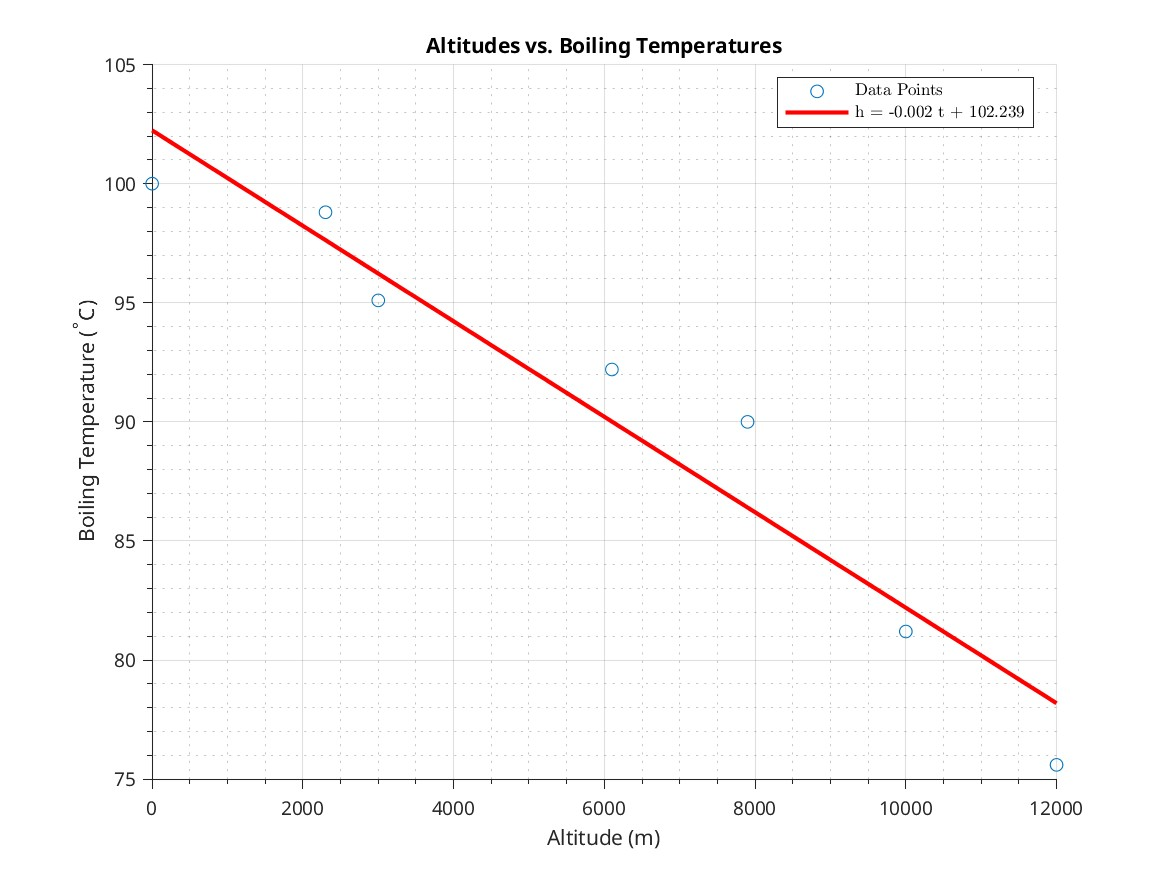
\includegraphics[width=1\textwidth]{main/graphs_images/altitudes_vs_boiling_temperatures.jpeg}
\begin{center}
    
\includegraphics[width=0.6\textwidth]{main/graphs_images/1screen.png}
\end{center}
It's hard to provide input for this type of data-related question.
You could consider adding altitude (\(h\)) as an input to determine the resulting boiling temperature (\(T_b\)).
 


\newpage

\begin{tcolorbox}[title={\color{black}\section{Q2}}, colback=white, colframe=\ni, boxrule=1mm, width=1\textwidth]
    The standard air density, \({D}\), at different heights, \({h}\), from sea level up to a height of \(33 \, \text{km}\) is given below:
    
    \[
    \begin{array}{|c|c|}
        \hline
        \textbf{Height (km)} & \textbf{Density (kg/m\(^3\))} \\ \hline
        0 & 1.2 \\ 
        3 & 0.91 \\ 
        6 & 0.66 \\ 
        9 & 0.47 \\ 
        12 & 0.31 \\ 
        15 & 0.19 \\ 
        18 & 0.12 \\ 
        21 & 0.075 \\ 
        24 & 0.046 \\ 
        27 & 0.029 \\ 
        30 & 0.018 \\ 
        33 & 0.011 \\ \hline
    \end{array}
    \]
    
    Make the following four plots of the data points (\({D}\) as a function of \({h}\)) on the same figure:
    
    \begin{enumerate}
        \item Both axes with linear scale.
        \item \({h}\) with log axis, \({D}\) with linear axis.
        \item \({h}\) with linear axis, \({D}\) with log axis.
        \item Both axes with log scale.
    \end{enumerate}
    
    Based on the plots, choose a function (linear, power, exponential, or logarithmic) that best fits the data points and determine its coefficients. Plot the function and the points using linear axes.
\end{tcolorbox}

\lstinputlisting[style=matlab, title=\textbf{\textcolor{\link}{\texttt{\href{https://github.com/sakx7/mathcompuni2/blob/main/main/q2.m}{main/q2.m}}}}]{main/q2.m}

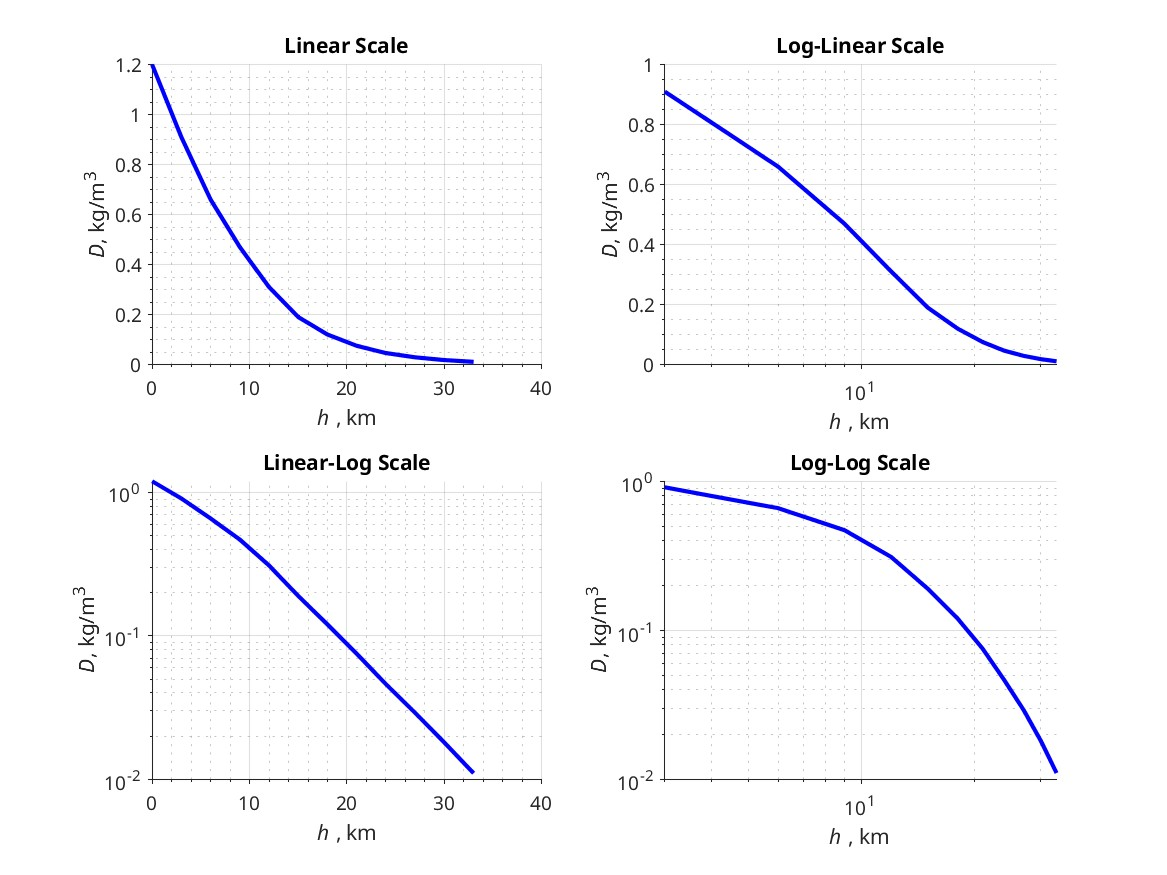
\includegraphics[width=1\textwidth]{main/graphs_images/subplts.jpeg}
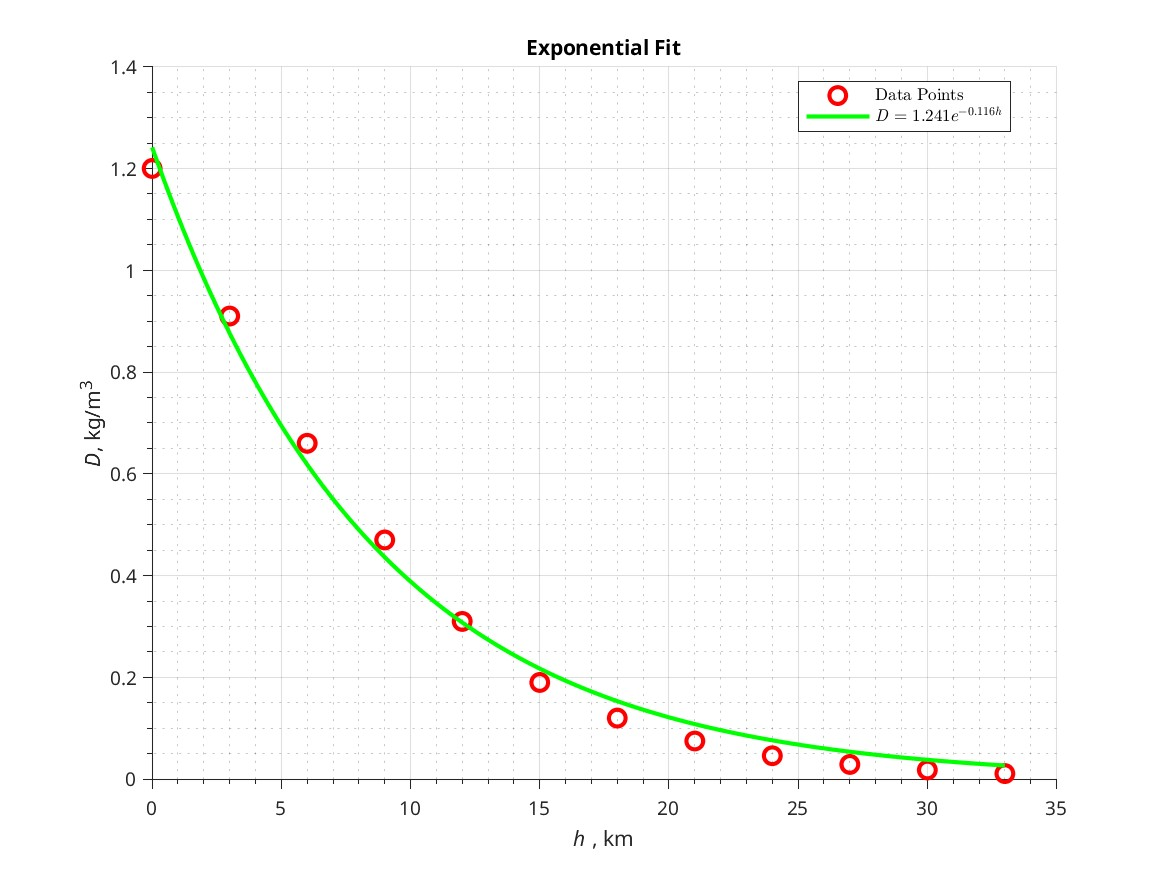
\includegraphics[width=1\textwidth]{main/graphs_images/fitted_curve.jpeg}
\begin{center}
    
\includegraphics[width=0.4\textwidth]{main/graphs_images/2screen.png}
\end{center}
Again it's hard to provide input for this type of data-related question. You could consider adding height (\(h\)) as an input to determine the resulting density (\(D\)).


\newpage

\begin{tcolorbox}[title={\color{black}\section{Q3}}, colback=white, colframe=\ni, boxrule=1mm, width=1\textwidth]
    Damped free vibrations can be modeled by a block of mass \((m)\) attached to a spring and a dashpot as shown.\vspace{-1em}
    \begin{center}
        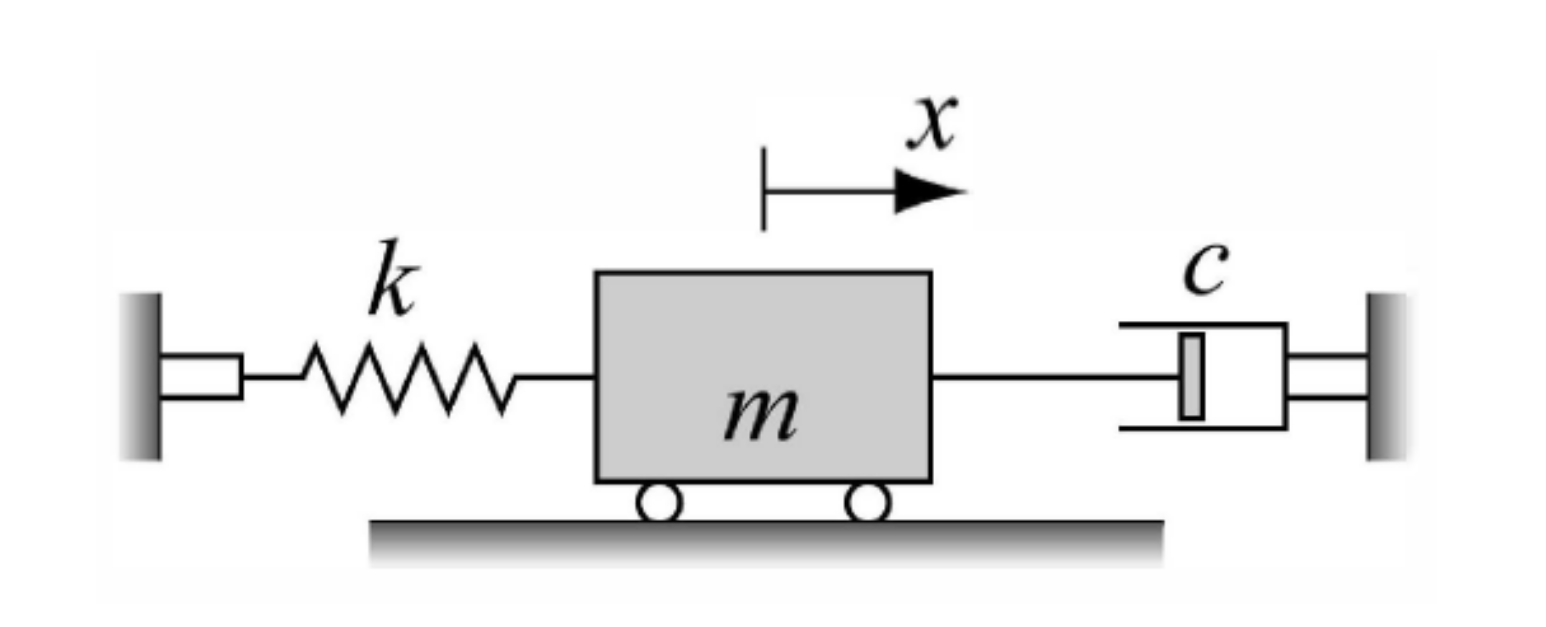
\includegraphics[width=0.7\textwidth]{main/graphs_images/3q.png}
    \end{center}
    From Newton's second law of motion, the displacement \(\mathbf{x}\) of the mass as a function of time can be determined by solving the differential equation:
    \[m \frac{d^2x}{dt^2} + c \frac{dx}{dt} + kx = 0\]
    where \(k\) is the spring constant and \(c\) is the damping coefficient. If the mass is displaced from its equilibrium position and released, it will oscillate back and forth. The nature of the oscillations depends on the values of \(m\), \(k\), and \(c\).\\[8pt]
    For the system shown, \(m = 10 \, \text{kg}\) and \(k = 28 \, \text{N/m}\). At \(t = 0\), the mass is displaced to \(x = 0.18 \, \text{m}\) and released from rest. Derive expressions for the displacement \(x(t)\) and velocity \(v(t)\), considering the following cases:
    \begin{enumerate}
        \item \(c = 3 \, \text{Ns/m}\), \(0 \leq t \leq 20 \, \text{s}\),
        \item \(c = 50 \, \text{Ns/m}\), \(0 \leq t \leq 10 \, \text{s}\).
    \end{enumerate}
    For each case, plot \(x(t)\) and \(v(t)\) versus \(t\) (two plots on one page).
\end{tcolorbox}

\lstinputlisting[style=matlab, title=\textbf{\textcolor{\link}{\texttt{\href{https://github.com/sakx7/mathcompuni2/blob/main/main/q3.m}{main/q3.m}}}}]{main/q3.m}
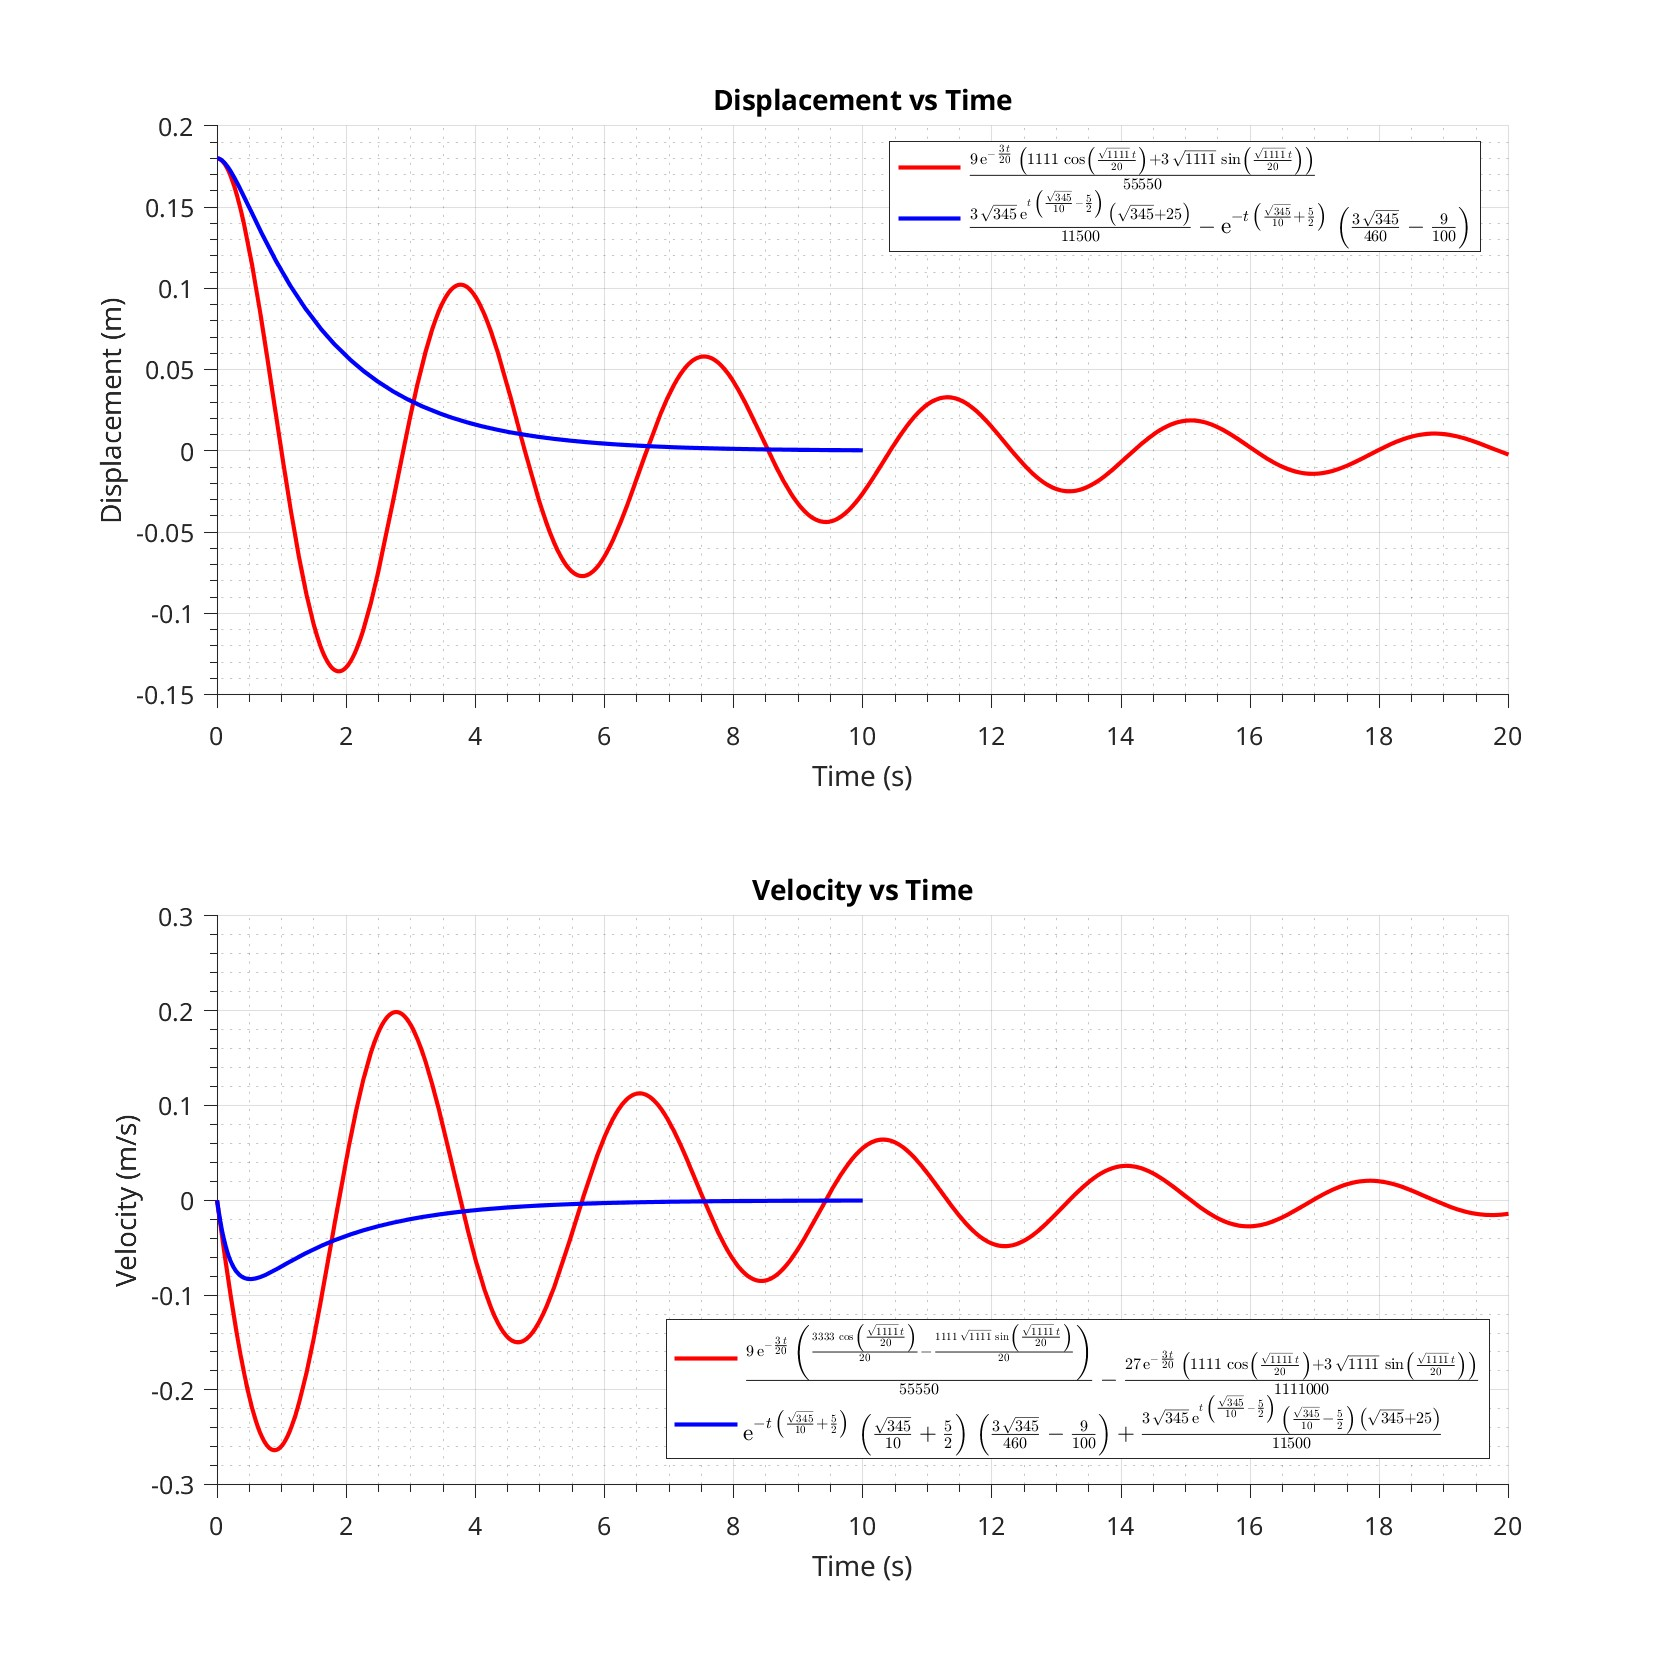
\includegraphics[width=1\textwidth]{main/graphs_images/damped_oscillation.jpeg}
\begin{center}
    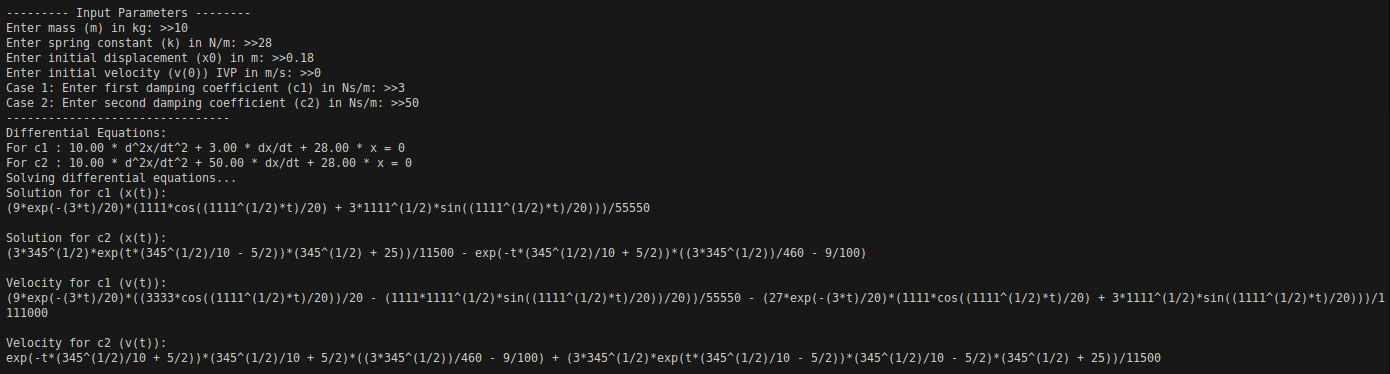
\includegraphics[width=1\textwidth]{main/graphs_images/3screen.png}
\end{center}
\newpage
    \begin{enumerate}[itemsep=1em,label=\textbf{\arabic*.}]
    \item \(\bm{c = 3} \, \textbf{Ns/m}\), \(\bm{0 \leq t \leq 20} \, \textbf{s}\),
        \[x(t) = \frac{9 e^{-\frac{3t}{20}} \left( 1111 \cos\left(\frac{\sqrt{1111} t}{20}\right) + 3 \sqrt{1111} \sin\left(\frac{\sqrt{1111} t}{20}\right) \right)}{55550}\]
        \[v(t) = \frac{9 e^{-\frac{3t}{20}} \left( \frac{3333 \cos\left(\frac{\sqrt{1111} t}{20}\right)}{20} - \frac{1111\sqrt{1111} \sin\left(\frac{\sqrt{1111} t}{20}\right)}{20} \right)}{55550} - \frac{27 e^{-\frac{3t}{20}} \left( 1111 \cos\left(\frac{\sqrt{1111} t}{20}\right) + 3 \sqrt{1111} \sin\left(\frac{\sqrt{1111} t}{20}\right) \right)}{1111000}\]\\[1.5em]
        This has been plotted on the graph within the respective range \({0 \leq t \leq 20} \, \text{s}\)
    \item \(\bm{c = 50} \, \textbf{Ns/m}\), \(\bm{0 \leq t \leq 10} \, \textbf{s}\).
        \[x(t) = \frac{3 \sqrt{345} e^{t\left(\frac{\sqrt{345}}{10} - \frac{5}{2}\right)} \left( \sqrt{345} + 25 \right)}{11500} - e^{-t\left(\frac{\sqrt{345}}{10} + \frac{5}{2}\right)} \left( \frac{3\sqrt{345}}{460} - \frac{9}{100} \right)\]
        \[v(t) = e^{-t\left(\frac{\sqrt{345}}{10} + \frac{5}{2}\right)}\left(\frac{\sqrt{345}}{10} + \frac{5}{2}\right)\left( \frac{3\sqrt{345}}{460} - \frac{9}{100} \right) + \frac{3\sqrt{345} e^{t\left(\frac{\sqrt{345}}{10} - \frac{5}{2}\right)}\left(\frac{\sqrt{345}}{10} - \frac{5}{2}\right)\left(345^{1/2} + 25\right)} {11500}\]\\[1.5em]
        This has been plotted on the graph within the respective range \({0 \leq t \leq 10} \, \text{s}\)
\end{enumerate}



\newpage

\begin{tcolorbox}[title={\color{black}\section{Q4}}, colback=white, colframe=\ni, boxrule=1mm, width=1\textwidth]\centering
    The currents \({i_1}\), \({i_2}\), and \({i_3}\) in the circuit are described by the equation set:
    \[\begin{pmatrix}
        2R & -R & 0 \\
        -R & 3R & -R \\
        0 & -R & 2R
    \end{pmatrix}
    \begin{pmatrix}
        i_1 \\ i_2 \\ i_3
    \end{pmatrix}
    =
    \begin{pmatrix}
        v_1 \\ 0 \\ v_2
    \end{pmatrix}\]
    Here, \(v_1\) and \(v_2\) are applied voltages. The other two currents can be found as:
    \[i_4 = i_1 - i_2, \quad i_5 = i_2 - i_3.\]
    \begin{center}
        \hspace{0.4em}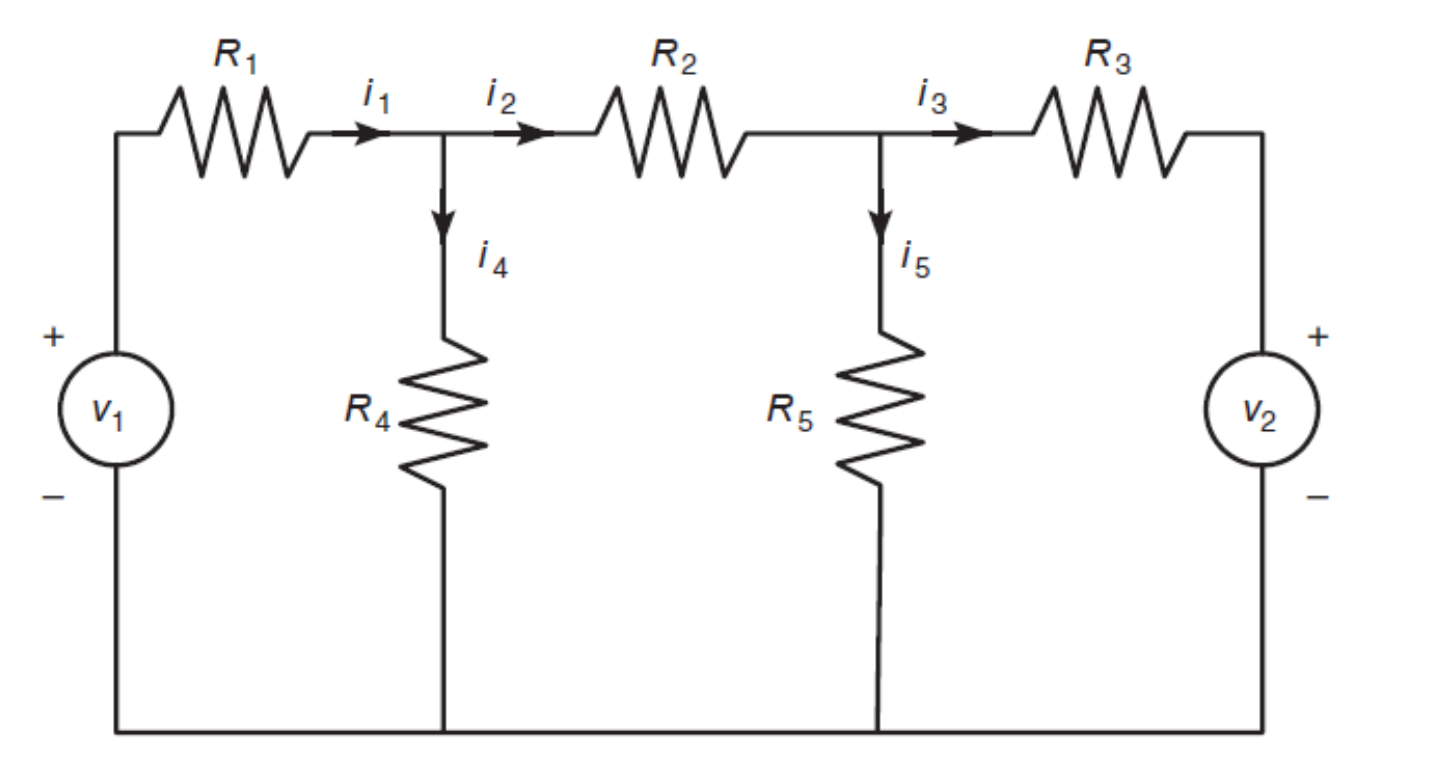
\includegraphics[width=0.7\textwidth]{main/graphs_images/4q.png}
    \end{center}
    \begin{enumerate}
        \item Use both the matrix inverse and division methods to solve for the currents in terms of \(R\), \(v_1\), and \(v_2\).
        \item Calculate the numerical values for the currents when \(R = 1000 \, \Omega\), \(v_1 = 100 \, \text{V}\), and \(v_2 = 25 \, \text{V}\).
    \end{enumerate}
\end{tcolorbox}
\raggedright
When i hear division i think of Cramer's rule, to calculate the currents (\(i_n\)) in a system of linear equations using Cramer's Rule, I used the following method in MATLAB. Cramer's Rule states:
\[i_n = \frac{\det(A_n)}{\det(A)}\]
Here:
\begin{itemize}[itemsep=-1mm]
    \item \(A\) is the coefficient matrix representing the system of linear equations.
    \item \(A_n\) is the matrix obtained by replacing the \(n\)-th column of \(A\) with the constant vector \(b\), which represents the applied voltages or external influences.
\end{itemize}
To compute this programmatically:
\begin{enumerate}[itemsep=-1mm]
    \item I first calculated the determinant of the original matrix \(A\) (denoted as \(\Delta_0\)) using the \code{det} function in MATLAB.
    \item Then, I used a \code{for} loop to iterate through each column of the matrix:
    \begin{itemize}[itemsep=-1mm]
        \item For each iteration \(k\), I created a modified version of \(A\) (denoted as \texttt{mNAM}) where the \(k\)-th column was replaced with the constant vector \(b\).
        \item I computed the determinant of the modified matrix (\(\Delta_k\)).
        \item Using Cramer's Rule, I calculated the current \(i_k = \frac{\Delta_k}{\Delta_0}\) and stored it in the array \texttt{I}.
    \end{itemize}
\end{enumerate}
For the inverse method, I interpret the solution as:
\[i_n = A^{-1} \cdot b\]
In this case, I utilize MATLAB's built-in function \code{inv} to compute the inverse of matrix \((A^{-1})\). It’s important to note that I define these matrices explicitly in my calculations before proceeding both methods.

\lstinputlisting[style=matlab, title=\textbf{\textcolor{\link}{\texttt{\href{https://github.com/sakx7/mathcompuni2/blob/main/main/q4.m}{main/q4.m}}}}]{main/q4.m}
\begin{center}
    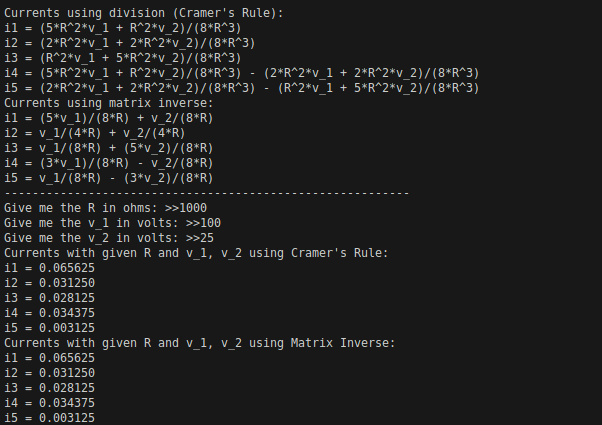
\includegraphics[width=1\textwidth]{main/graphs_images/4screen.png}
\end{center}

\begin{minipage}{0.5\textwidth}\centering
    \textbf{Currents using division (Cramer's Rule):}
    \[i_1 = \frac{5R^2v_1 + R^2v_2}{8R^3}\]
    \[i_2 = \frac{2R^2v_1 + 2R^2v_2}{8R^3}\]
    \[i_3 = \frac{R^2v_1 + 5R^2v_2}{8R^3}\]
    \[i_4 = \frac{5R^2v_1 + R^2v_2}{8R^3} - \frac{2R^2v_1 + 2R^2v_2}{8R^3}\]
    \[i_5 = \frac{2R^2v_1 + 2R^2v_2}{8R^3} - \frac{R^2v_1 + 5R^2v_2}{8R^3}\]
\end{minipage}\hfill%
\begin{minipage}{0.45\textwidth}\centering
    \textbf{Currents using matrix inverse:}
    \[i_1 = \frac{5v_1}{8R} + \frac{v_2}{8R}\]
    \[i_2 = \frac{v_1}{4R} + \frac{v_2}{4R}\]
    \[i_3 = \frac{v_1}{8R} + \frac{5v_2}{8R}\]
    \[i_4 = \frac{3v_1}{8R} - \frac{v_2}{8R}\]
    \[i_5 = \frac{v_1}{8R} - \frac{3v_2}{8R}\]
\end{minipage}\\[1em]
\begin{center}
\textbf{Given the following values:} , $R = 1000 \, \Omega$, $v_1 = 100 \, \text{V}$, $v_2 = 25 \, \text{V}$
\end{center}
\vspace{-1em}
\begin{minipage}{0.45\textwidth}\centering
    \[i_1 = 0.065625\]
    \[i_2 = 0.031250\]
    \[i_3 = 0.028125\]
    \[i_4 = 0.034375\]
    \[i_5 = 0.003125\]
\end{minipage}\hfill%
\begin{minipage}{0.45\textwidth}
    \[i_1 = 0.065625\]
    \[i_2 = 0.031250\]
    \[i_3 = 0.028125\]
    \[i_4 = 0.034375\]
    \[i_5 = 0.003125\]
\end{minipage}\\[1em]

The numerical values are identical, as can also be observed from the equations, which are equivalent in each case.

\end{document}

